\documentclass{standalone}
\usepackage{tikz}
\usetikzlibrary{positioning, shapes, arrows.meta}

\begin{document}
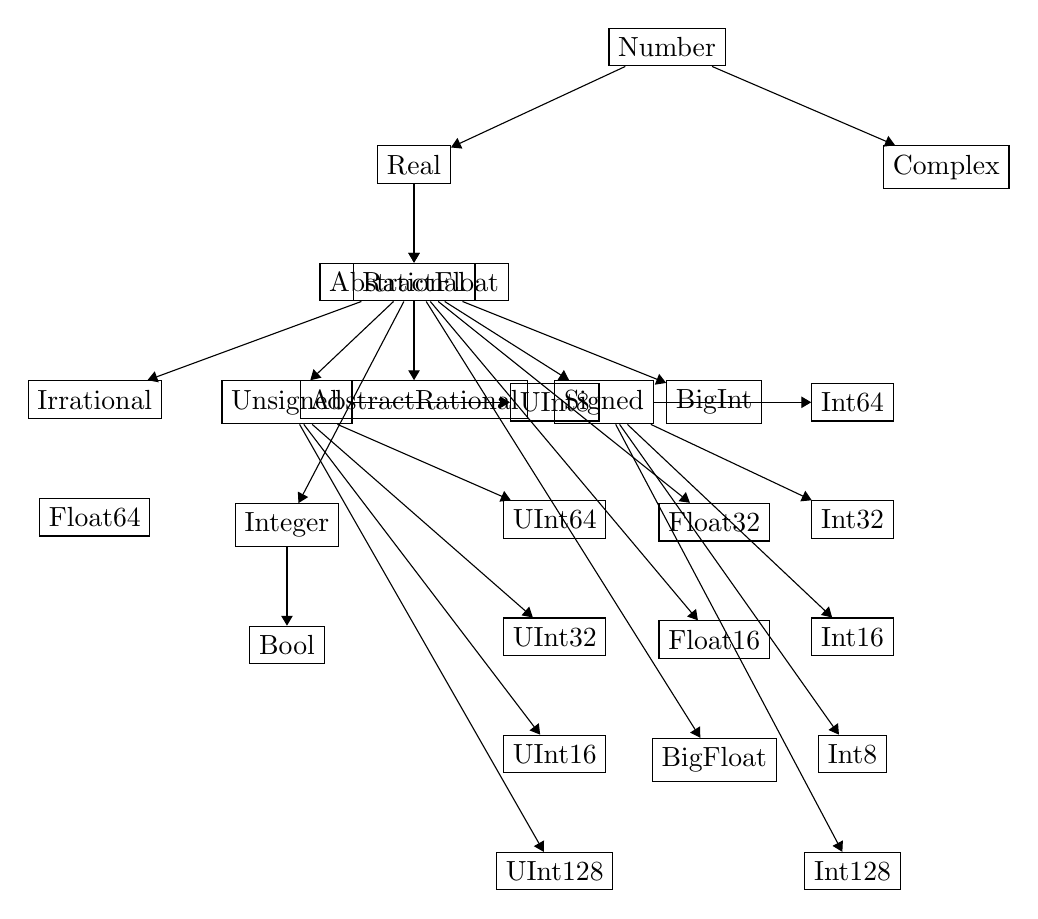
\begin{tikzpicture}[
    node distance=1cm and 2cm,
    mynode/.style={rectangle, draw, align=center},
    myarrow/.style={-Triangle}]

    \node[mynode] (number) {Number};
    \node[mynode, below left=of number] (real) {Real};
\node[mynode, below right=of number] (complex) {Complex};    
	
    \node[mynode, below=of real] (rational) {Rational};
    \node[mynode, below left=of rational, xshift=2cm] (unsigned) {Unsigned};
    \node[mynode, below right=of rational, xshift=-1cm] (signed) {Signed};

    \draw[myarrow] (number) -- (real);
    \draw[myarrow] (real) -- (rational);
    \draw[myarrow] (rational) -- (unsigned);
    \draw[myarrow] (rational) -- (signed);

    \node[mynode, right=of unsigned] (uint8) {UInt8};
    \node[mynode, below=of uint8] (uint64) {UInt64};
    \node[mynode, below=of uint64] (uint32) {UInt32};
    \node[mynode, below=of uint32] (uint16) {UInt16};
    \node[mynode, below=of uint16] (uint128) {UInt128};

    \node[mynode, right=of signed] (int64) {Int64};
    \node[mynode, below=of int64] (int32) {Int32};
    \node[mynode, below=of int32] (int16) {Int16};
    \node[mynode, below=of int16] (int8) {Int8};
    \node[mynode, below=of int8] (int128) {Int128};

    \draw[myarrow] (unsigned) -- (uint8);
    \draw[myarrow] (unsigned) -- (uint64);
    \draw[myarrow] (unsigned) -- (uint32);
    \draw[myarrow] (unsigned) -- (uint16);
    \draw[myarrow] (unsigned) -- (uint128);

    \draw[myarrow] (signed) -- (int64);
    \draw[myarrow] (signed) -- (int32);
    \draw[myarrow] (signed) -- (int16);
    \draw[myarrow] (signed) -- (int8);
    \draw[myarrow] (signed) -- (int128);

    \node[mynode, below=of unsigned] (integer) {Integer};
    \node[mynode, below=of integer] (bool) {Bool};
    \node[mynode, below=of rational] (abstractrational) {AbstractRational};
    \node[mynode, below=of real] (abstractfloat) {AbstractFloat};
    \node[mynode, below left=of abstractfloat] (irrational) {Irrational};
    \node[mynode, below=of irrational] (float64) {Float64};
    \node[mynode, below right=of abstractfloat] (bigint) {BigInt};
    \node[mynode, below=of bigint] (float32) {Float32};
    \node[mynode, below=of float32] (float16) {Float16};
    \node[mynode, below=of float16] (bigfloat) {BigFloat};
    

    \draw[myarrow] (rational) -- (integer);
    \draw[myarrow] (integer) -- (bool);
    \draw[myarrow] (rational) -- (abstractrational);
    \draw[myarrow] (real) -- (abstractfloat);
    \draw[myarrow] (abstractfloat) -- (irrational);
    \draw[myarrow] (abstractfloat) -- (bigint);
    \draw[myarrow] (abstractfloat) -- (float32);
    \draw[myarrow] (abstractfloat) -- (float16);
    \draw[myarrow] (abstractfloat) -- (bigfloat);
    \draw[myarrow] (number) -- (complex);

\end{tikzpicture}
\end{document}
